\documentclass[landscape,a1paper, fontscale=0.35]{baposter}
\usepackage[linesnumbered,ruled,vlined]{algorithm2e}
\SetAlFnt{\footnotesize}
\SetAlgoLined
\SetAlCapFnt{\small}
\SetAlCapNameFnt{\small}
\setlength{\algomargin}{1em}
\usepackage{tikz}
\usepackage{graphicx}
\usepackage{caption}
\usepackage{lettrine}
\usepackage{subcaption}
\usepackage{palatino}
\usetikzlibrary{shapes,arrows,positioning,calc}
%%%%%%%%%%%%%%%%%%%%%%%%%%%%%%%%%%%%%%%%%%%%%%%%%%%%%%%%%%%%%%%%%%%%%%%%%%%%%%%%
% Save space in lists. Use this after the opening of the list
%%%%%%%%%%%%%%%%%%%%%%%%%%%%%%%%%%%%%%%%%%%%%%%%%%%%%%%%%%%%%%%%%%%%%%%%%%%%%%%%
\newcommand{\compresslist}{%
\setlength{\itemsep}{1pt}%
\setlength{\parskip}{0pt}%
\setlength{\parsep}{0pt}%
}

\newcommand{\clustertriangle}{%
    \begin{center}
    \vspace{1em}
    \begin{tikzpicture}
        \node (spiderman) at (3,2)
        {\pgfbox[center, bottom]
            {\pgftext{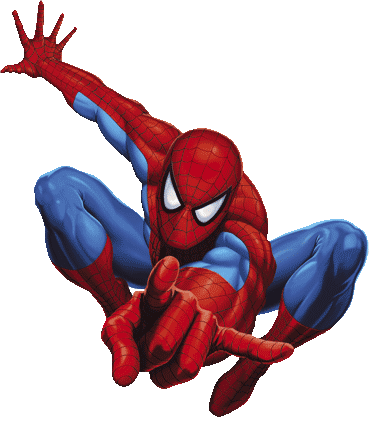
\includegraphics[height=5em]{images/spiderman.png}}}};
            \node (wolverine) at (1, 0)
        {\pgfbox[center, bottom]
            {\pgftext{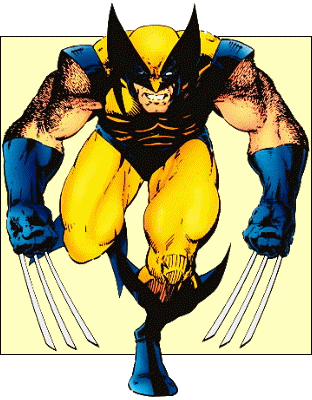
\includegraphics[height=5em]{images/wolverine.png}}}};
        \node (modok) at (5, 0)
        {\pgfbox[center, bottom]
            {\pgftext{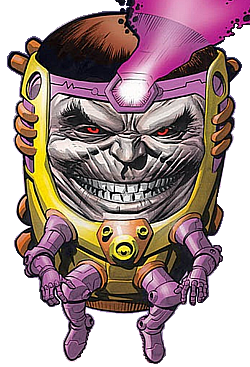
\includegraphics[height=5em]{images/modok.png}}}};
            \draw[-, dotted] (spiderman) -- node {link} (wolverine);
            \draw[-, dotted] (wolverine) -- node {link} (modok);
            \draw[-, dotted] (modok)     -- node {?} (spiderman);
    \end{tikzpicture}
    \vspace{1em}
\end{center}
}

\newcommand{\roulette}{%
\begin{tikzpicture}[scale=3]
    \vspace{1em}
\draw[dashed] (0cm, 0cm) circle(1cm);
\foreach \x/\y/\xcolour/\xopacity/\ximage/\xz/\xsize in {
    0/90/blue/0.5/spiderman/45/6em,
    280/360/blue/0.4/wolverine/310/5em,
    280/210/blue/0.3/modok/240/4em,
    210/140/blue/0.25/doom/180/4em,
    140/110/blue/0.2/ironman/120/2.5em,
    110/100/blue/0.15/hulk/105/1em,
    100/90/blue/0.1/thing/95/0.5em}
{
\filldraw[fill=\xcolour,draw=black, fill opacity=\xopacity](0:0cm) -- (\x:1cm)
arc (\x:\y:1cm) -- cycle;
\draw (\xz:0.6cm) node (\ximage) {\pgfbox[center, bottom]{
    \pgftext{\includegraphics[height=\xsize]{images/\ximage}}}};
}

\end{tikzpicture}
}

\newcommand{\approximation}{%
    \begin{minipage}[t]{0.45\textwidth}
            \vspace{0pt}
            \centering
        \begin{algorithm}[H]
            \SetAlgoLined
            \DontPrintSemicolon
            \KwIn{An integer $k$ and a network $N = \left(V,E\right)$ of $n$ nodes}
            \KwOut{An approximation of the clustering coefficient $\hat{C}_{N}$}
            $c \gets 0$\\
            \For{$i \gets 0$ $\mathbf{to}$ $k$}
            {
            $j \gets\mathtt{\small UniformRandomNode}\left(\right)$\\
            $u \gets\mathtt{\small UnifromRandomNeighbour}\left(j\right)$\\
            \Repeat{$u \neq v$}
            {
                $v \gets \mathtt{\small UniformRandomNeighbour}\left(u\right)$\\
            }
            \If{$\mathtt{\small EdgeExists}\left(i, v\right)$}
            {
                $c \gets c + 1$\\
            }
            }%
            \KwRet{$c / k$}%
            \caption{Schank-Wagner}%
        \end{algorithm}%
    \end{minipage}%
}

\newcommand{\iterator}{%
    \begin{minipage}[t]{0.45\textwidth}
        \vspace{0pt}
        \centering
\begin{algorithm}[H]
\SetAlgoLined
                \KwIn{A network $N = (V, E)$, with $n$ nodes}
                \KwOut{The clustering coefficient $C_{N}$}
                $c \gets 0$\\
                \For{$i \in V$}
                {
                    $d \gets i.\mathrm{degree}$\\
                    $e \gets 0$\\
                    \For{$j \in i.\mathrm{neighbours}$}
                    {
                        \For{$k \in j.\mathrm{neighbours}$}
                        {
                            \If {$\mathtt{IsNeighbour}\left(i,j\right)$}
                            {
                                $e \gets e + 1$
                            }
                        }
                    }
                    $c \gets e / \left(d\left(d-1\right)\right)$
                }%
                \KwRet{$c / n $}%
                \caption{NODE-ITERATOR}%
            \end{algorithm}%
        \end{minipage}%
        }
\begin{document}
\definecolor{lightblue}{rgb}{0.145,0.6666,1}
\begin{poster}
    % Poster options
    {
        background=plain,
        bgColorOne=white,
        bgColorTwo=white,
        borderColor=lightblue,
        headerColorOne=blue,
        headerColorTwo=lightblue,
        headerFontColor=white,
        boxColorOne=white,
        boxColorTwo=lightblue,
        eyecatcher=true,
        headerborder=closed,
        headerheight=0.11\textheight,
      headerborder=closed,
      textfont={\setlength{\parindent}{1.5em}}
    }
{
    
\includegraphics[height=3.0em]{images/marvel.png}
}
{
    \LARGE Computing the Clustering Coefficient in Scale-free Networks
}
{
    Yegor Guskov, Lloyd Henning, Jacobus Meulen, Peter Sutton\\
    {\small\tt\{guskov9, henninl8, meulen9, suttonp8\}@cs.man.ac.uk}
}
{
    
\includegraphics[height=3.0em]{images/logo}
}
%%%%%%%%%%%%%%%%%%%%%%%%%%%%%%%%%%%%%%%%%%%%%%%%%%%%%%%%%%%%%%%%%%%%%%%%%%%%%%%
% Content begins
%%%%%%%%%%%%%%%%%%%%%%%%%%%%%%%%%%%%%%%%%%%%%%%%%%%%%%%%%%%%%%%%%%%%%%%%%%%%%%%
\headerbox{Introduction}{name=problem,column=0,row=0}
{
    \lettrine{W}{e} present methods for computing the clustering coefficient of a
    scale-free network.

}
%%%%%%%%%%%%%%%%%%%%%%%%%%%%%%%%%%%%%%%%%%%%%%%%%%%%%%%%%%%%%%%%%%%%%%%%%%%%%%%
\headerbox{Clustering Coefficient}{name=clustering, column=0, below=problem}
{
    \lettrine{G}{iven} a network $N = \left(V, E\right)$  of $n$ nodes with links $\left(u, v\right),
    \left(v, w\right) \in E$, the clustering coefficient $C_{N}$ gives the
    likeliness of $\left(u, w\right) \in E$.

    Intuitively, it answers the question,``If Spiderman has appeared in the
    same comic as Wolverine and Wolverine has appeared in the same comic as
    M.O.D.O.K., how likely is it that Spiderman and M.O.D.O.K. have
    appeared in the same comic?''.\\
    \clustertriangle
    \vspace{0.5em}
    We define $C_{N}$ as
    \[
        C_{N} = \frac{1}{n} \displaystyle\sum_{i}
            {\frac{2e_{i}}{k_{i}\left(k_{i} -1\right)}}
    \]
    where $k_{i}$ is the number of neighbours of the $i$th node and $e_{i}$ is
    the number of links shared between the neighbours of the $i$th node.
    \vspace{-0.5em}
}
%%%%%%%%%%%%%%%%%%%%%%%%%%%%%%%%%%%%%%%%%%%%%%%%%%%%%%%%%%%%%%%%%%%%%%%%%%%%%%
\headerbox{Barab\'{a}si-Albert model}{name=bamodel, column=1, row=0}
{
    \lettrine{T}{he} Barab\'{a}si-Albert (BA) model is a model of scale-free networks.
    Networks are grown by adding new nodes with links established between them
    by \emph{preferential attachment}.

    To generate a BA model, we start with an initial network $N$ of
    $n_{0}$ nodes. Then for each timestep $t \leq T$ we add a new node $u$ to
    the graph and links $\left(u, i\right)$ where $i$ has degree $k_{i}$ and is
    selected from the existing nodes with probability
    \[
        \Pi\left(k_{i}\right) =
        \frac{k_{i}}{\displaystyle\sum_{j}{k_{j}}}.
    \]
    Preferential attachment is best seen as a roulette wheel, where
    the size of the slots is proportional to the degree of the associated node.\\
    \noindent\roulette
    \captionof{figure}{A visualisation of preferential attachment where
        Spiderman has the greatest degree and therefore is the most likely to be
    \emph{attached} to new nodes.}
}

%%%%%%%%%%%%%%%%%%%%%%%%%%%%%%%%%%%%%%%%%%%%%%%%%%%%%%%%%%%%%%%%%%%%%%%%%%%%%%
\headerbox{Experimental Results}{name=results, column=2, span=2, row=0}
{
    \begin{center}
        \begin{minipage}[t]{1\textwidth}
    \begin{minipage}[t]{0.49\textwidth}
        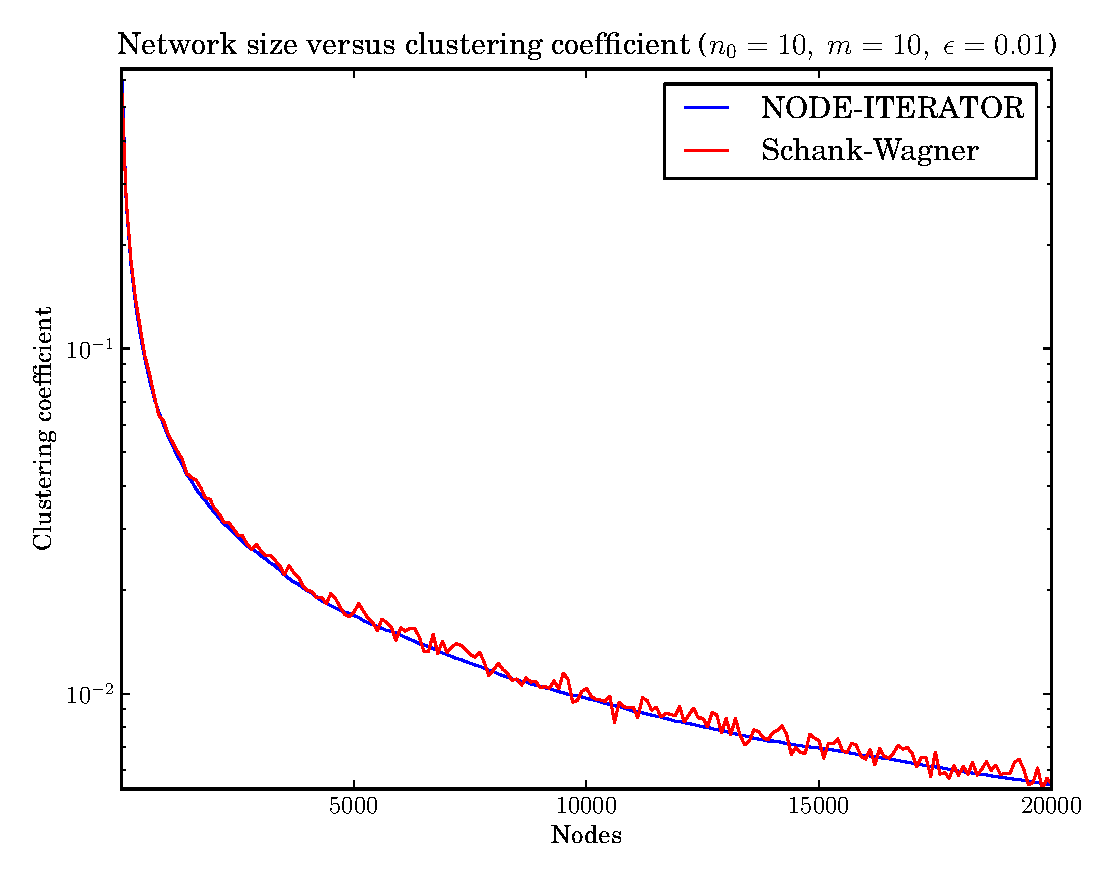
\includegraphics[height=15em]{images/cc.eps}
        \captionof{figure}[a]{Clustering coefficient}
    \end{minipage}
    \null
    \hfill
    \null
    \begin{minipage}[t]{0.49\textwidth}
        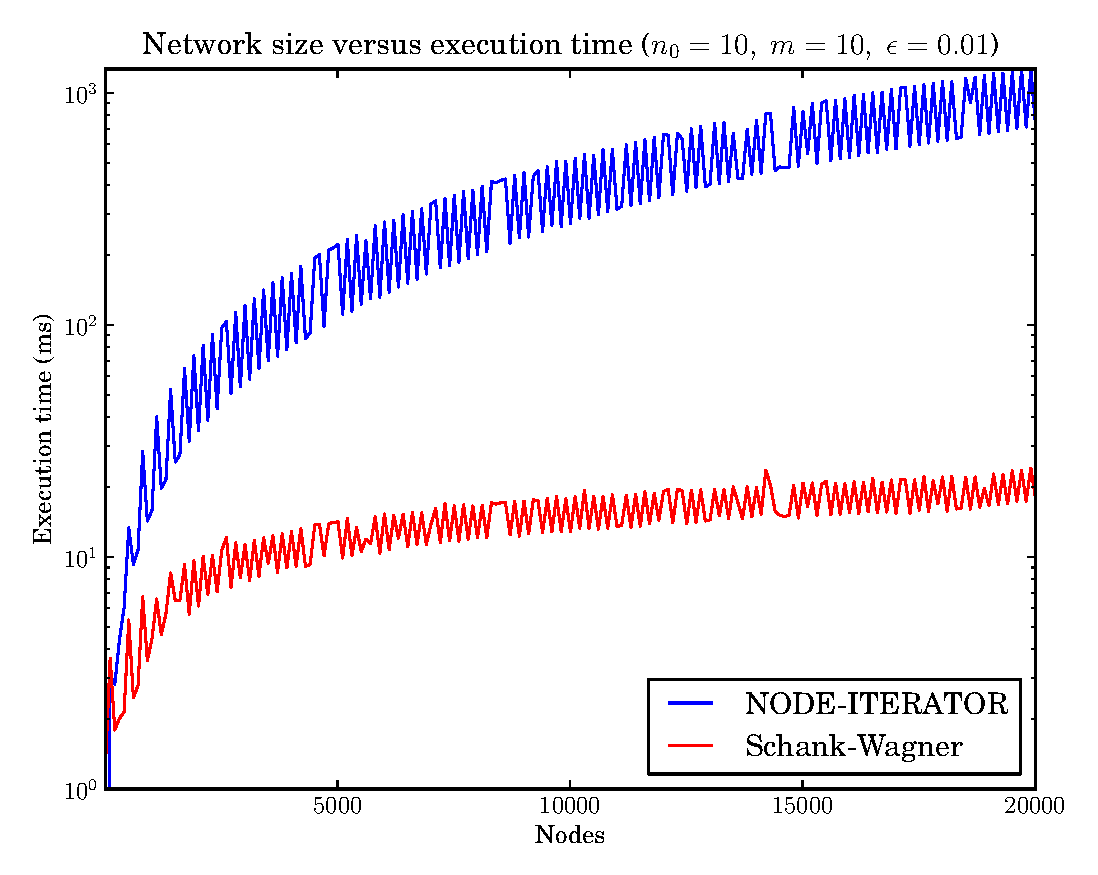
\includegraphics[height=15em]{images/time.eps}
        \captionof{figure}[b]{Execution time}
    \end{minipage}
    \hfill
    \null
    \end{minipage}
\end{center}
}
%%%%%%%%%%%%%%%%%%%%%%%%%%%%%%%%%%%%%%%%%%%%%%%%%%%%%%%%%%%%%%%%%%%%%%%%%%%%%%
\headerbox{Polynomial and Sublinear Approaches}{name=exact-algorithm,
below=results ,column=2,span=2}
{
    \lettrine{T}{he} algorithms below compute the clustering coefficient $C_{N}$
    of a network $N$. Algorithm 1 computes $C_{N}$ exactly and Algorithm 2
    computes an approximation.

    \vspace{-1em}
    \null\hspace{-1em}
    \iterator\hspace{1em}
    \approximation
    \null\hfill\\\\
    For a network of $n$ nodes, such that the greatest node degree is $d$, the
    time complexity of NODE-ITERATOR and Schank-Wagner is
    $\mathcal{O}\left(nd^{2}\right)$ and $\mathcal{O}\left(k\right)$
    respectively, where $k = \left\lceil
    \ln\left(2n\right)/2\epsilon^{2}\right\rceil$ and $\epsilon$ is the error
    bound.
}
%%%%%%%%%%%%%%%%%%%%%%%%%%%%%%%%%%%%%%%%%%%%%%%%%%%%%%%%%%%%%%%%%%%%%%%%%%%%%%
\headerbox{References}{name=references, column=0, below=clustering, above=bottom}
{
    \tiny
    \bibliographystyle{ieee}
    \renewcommand\refname{\vskip -0.7em}
    \begin{thebibliography}{1}
        \bibitem{Albert01:statisticalmechanics}
            R. Z. Albert and A. Barab\'{a}si
            \newblock{Statistical Mechanics Of Complex Networks},
            \newblock In {Reviews of Modern Physics, 2002, volume 74, page 47}
            \vspace{-1.7em}
        \bibitem{Schank05:approximatingclustering}
            T. Schank, D. Wagner.
            \newblock {Approximating clustering coefficient and
                        transitivity}
                        \newblock In {Journal of Graph Algorithms and
                        Applications, 2005, volume 9, page 2005}
    \end{thebibliography}
}
\end{poster}
\end{document}
